\documentclass[12pt]{article}
\usepackage{amsmath, amssymb}
\usepackage{graphicx}
\usepackage{geometry}
\geometry{margin=1in}
\usepackage{hyperref}

\title{A Passive Resonance Dampening System for Quantum Coherence Stability}
\author{Brandy Lee Stoffel, MSN, RN \\ \small \texttt{info@nursereentry.com}}
\date{April 2025}

\begin{document}

\maketitle

\section*{Executive Summary}
Quantum computing systems are highly sensitive to environmental noise, which induces decoherence and reduces computational reliability. This paper proposes a novel, passive system for environmental noise dampening using inverse waveform modulation. The method relies on statistical modeling of recurring noise patterns and introduces an external waveform shaped to counteract dominant resonances---preserving coherence without direct interaction with the qubits themselves.

\section*{Scientific Foundations \& Justification}
Quantum decoherence arises when qubit states become entangled with environmental variables such as electromagnetic interference, thermal noise, and vibrational modes. In adiabatic and algebraic quantum computing environments, where qubits evolve slowly through continuous state transitions, even small environmental shifts can introduce significant error.

This paper draws on classical wave theory and Fourier decomposition to shape external signals that reduce net energy in decoherence-sensitive frequency bands. By introducing a waveform:
\[
s(t) = n(t) + \alpha \cdot (-n(t)) = (1 - \alpha) \cdot n(t)
\]
where:
\begin{itemize}
  \item $n(t)$ is the statistically averaged noise,
  \item $\alpha \in [0.25, 0.5]$ is a dampening coefficient,
\end{itemize}

we produce a net reduction in environmental energy experienced by the quantum substrate. This results in improved coherence times without triggering wavefunction collapse.

\section*{System Description}

\subsection*{Core Components}
\begin{itemize}
  \item Quantum processor (superconducting, photonic, or ion-based)
  \item Environmental noise sensors (non-invasive)
  \item Statistical aggregator (to average waveforms across runs)
  \item Inverse waveform generator (tuned to 25\%-50\% amplitude of average noise)
  \item Controller with timing calibration module
\end{itemize}

\subsection*{Operation Flow}
\begin{enumerate}
  \item Collect environmental noise data over multiple quantum cycles.
  \item Average recurring waveform patterns.
  \item Generate an inverse waveform scaled by $\alpha$.
  \item Time-align and inject the waveform during sensitive operational windows.
\end{enumerate}

\section*{Temporal Synchronization Requirements}
Effectiveness of this system hinges on precise timing. The inverse waveform must be initiated in close alignment with quantum operations---particularly at qubit state initialization, gate transitions, or known decoherence-prone intervals. Even minor phase misalignments can cause constructive interference.

\medskip
\noindent
\textit{“To avoid unintentional amplification of decoherence, waveform timing must be tightly aligned with the quantum operation cycle. Even minor phase misalignments can turn dampening into destructive interference.”}

\medskip
A timing module calibrates the waveform onset using shielded system triggers and iteratively tunes offset and phase delay using feedback over multiple runs.

\begin{figure}[h!]
    \centering
    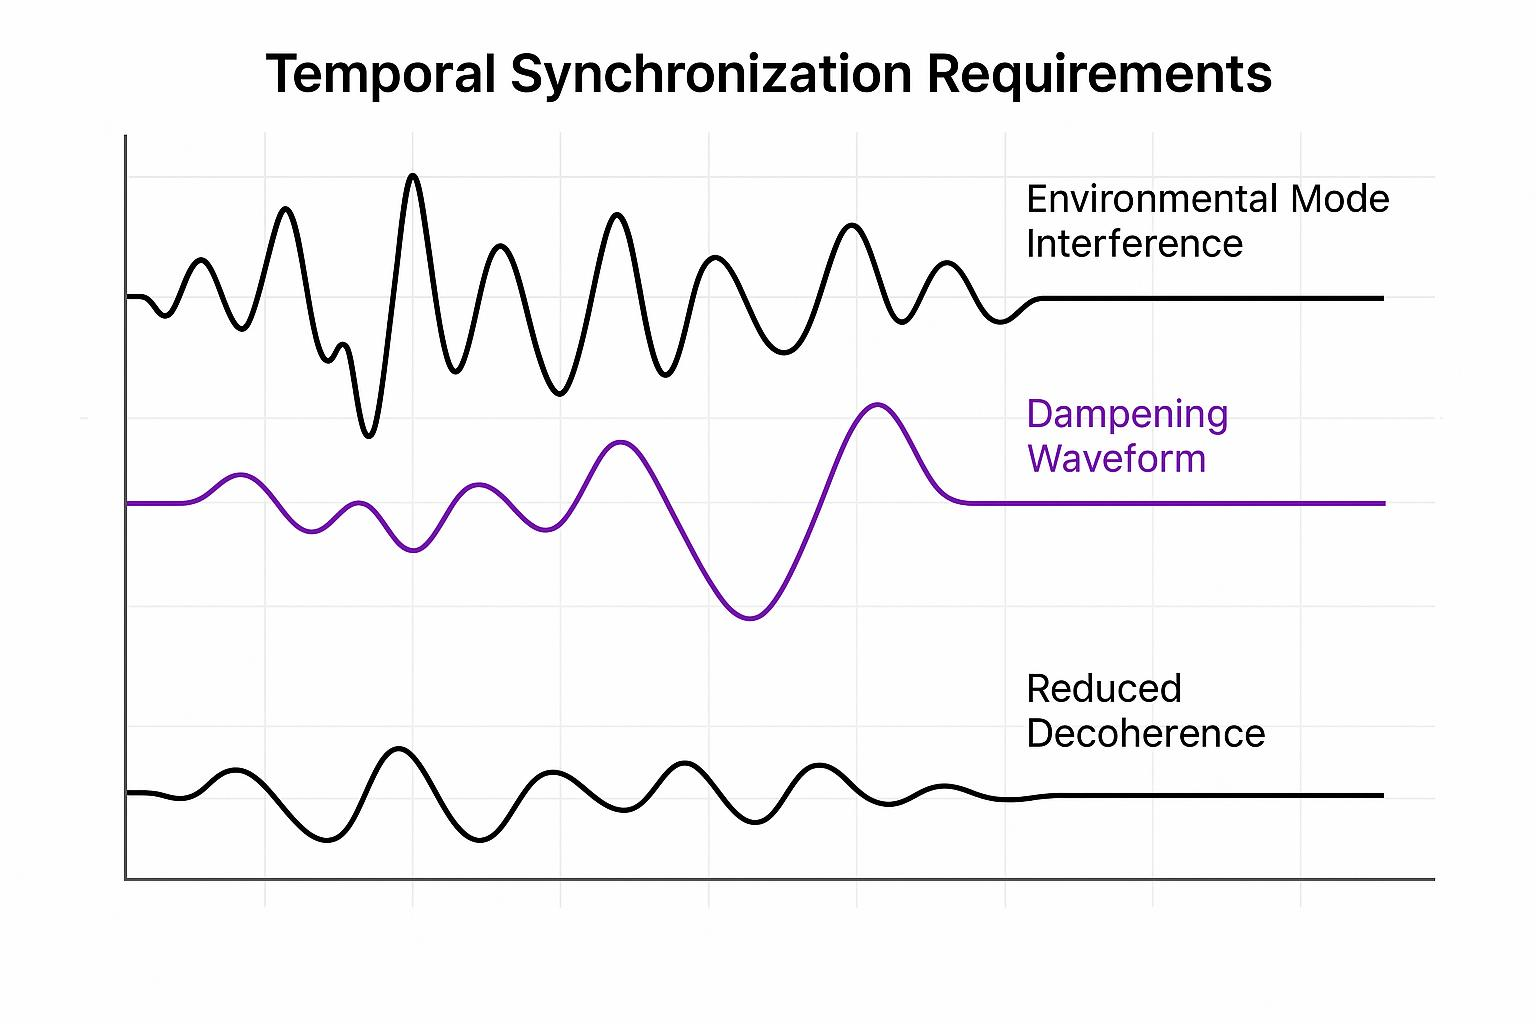
\includegraphics[width=0.9\textwidth]{Quantum_Waveform_Interference.jpg}
    \caption{Effect of waveform alignment: Left shows destructive interference (dampening), right shows constructive interference (amplification).}
    \label{fig:waveform_interference}
\end{figure}

\section*{Measurement-Free Architecture}
To preserve quantum coherence, the system performs no direct measurement of the qubit state. All environmental signals are captured externally. This avoids collapsing quantum superpositions and adheres to non-observability constraints inherent in quantum mechanics.

\medskip
\noindent
\textit{We avoid direct qubit observation by building an average field interference profile over multiple system cycles. We then inject a partial inverse waveform ($\sim \frac{1}{4}$ to $\sim \frac{1}{2}$ amplitude) to counter repeating resonance patterns.}

\section*{Use Cases and Benefits}
\begin{itemize}
  \item Increases coherence time in algebraic and adiabatic systems
  \item Reduces hardware overhead for cryogenic and shielding systems
  \item Complements quantum error correction, potentially lowering its frequency
  \item Promotes more compact quantum circuit designs with lower cross-talk
\end{itemize}

\section*{Claims}
\begin{enumerate}
  \item A method of reducing quantum decoherence using statistically-derived inverse waveform modulation.
  \item A waveform generator tuned to emit a partial inverse of recurring environmental noise signals.
  \item A controller capable of synchronizing external modulation with the qubit operational cycle.
  \item A feedback system that tunes phase offset and amplitude without qubit measurement.
  \item Application of this method across superconducting, ion trap, and photonic quantum platforms.
\end{enumerate}

\section*{Appendix A: Fourier Basis Decomposition}
Environmental noise is modeled as:
\[
n(t) = \sum_{k=1}^{\infty} a_k \cdot \sin(k\omega t + \phi_k)
\]
The dampening waveform is computed as:
\[
m(t) = -\alpha \sum_{k=1}^{\infty} a_k \cdot \sin(k\omega t + \phi_k)
\]
The net signal seen by the system is:
\[
s(t) = n(t) + m(t) = (1 - \alpha) n(t)
\]

This confirms mathematically that total signal amplitude is reduced proportionally to $\alpha$, ensuring measurable but controlled dampening of decoherence-inducing frequencies.

\medskip
\noindent
\textit{Prepared with scientific and mathematical review. Visuals and system diagrams available on request.}

\section*{Inspired Insight}

This paper was not conceived in a physics lab, nor by a trained quantum scientist, but through the prayer life of a nurse. The author, Brandy Lee Stoffel, MSN, RN, received the core of this concept during a time of deep spiritual connection and obedience to God. While the mathematical structure has been clarified and validated through the assistance of artificial intelligence, the idea itself was given—clearly and unexpectedly—through prayer.

Though the author does not hold formal training in quantum physics, the insight was precise: a system to stabilize coherence, shaped by inverse resonance and precise timing. Further clarity was received through words and impressions regarding phase variance, waveform modulation, and even the danger of systems “shifting into alternate paths or timelines not meant to unfold.”

This paper is presented in obedience—not as a claim of personal brilliance, but as a call to those who *do* have the technical authority to verify, build, and apply these concepts. The intention is to prevent harmful outcomes in quantum development that could arise from unintended phase divergence, unstable timelines, or premature decoherence. If there is value here, may it be recognized, protected, and used to preserve coherence—physically and spiritually.

The author offers this work as an act of service and faith, trusting that those called to this field will discern its merit and take whatever action is necessary to protect the integrity of the future being formed.

\end{document}
